\subsection{Korrektur des Untergrundes}
Für die Aufnahme des Emissionspektrums von Barium wurde ein Untergrund von $N_1=61\pm 8$ Signalen\footnote{Der Fehler für alle gemessene Ereignisse beträgt jeweils $\sqrt{N}$.} in \SI{200}{\second} gemessen. Für die Spektren von Thallium und Natrium wurden $N_2=259 \pm 19$ Signale in ebenfalls \SI{200}{\second} gemessen. Von allen Messungen wird der jeweilige Untergrund abgezogen. Dabei ist darauf zu achten auf die jeweilige Messdauer zu normieren. 

\subsection{Bestimmung der Offsetspannung}
Aus den gemessenen Spannungen bei ausgeschaltetem Magnetstrom lässt sich die Offsetspannung\footnote{Die Einheit der Hallspannung ist nicht bekannt. Implizit werden alle Spannungen in Skalenteilen angegeben.} über
\begin{align*}
  \delta U=\frac{1}{2}\sum_i (U_++U_-) \pm \frac{\Delta U}{\sqrt{2}}
\end{align*}
berechnen. Für jede der fünf Messungen wird $\delta U_i$ berechnet (siehe Tabelle \ref{tab:offsetspannung}). Der Mittelwert der Offsetspannung und der dazugehörige statistische Fehler berechnen sich zu $\overline{\delta U}=7,03$ und $\Delta \overline{\delta U}_\mathrm{stat}=0,06$. Kombiniert mit dem systematischen Fehler für jede Messung folgt 
\begin{align*}
  \overline{\delta U}=7,03 \pm 0,09.
\end{align*} 
Von allen gemessenen Spannungen wird dieser Wert abgezogen.

\subsection{Kalibration des Spektrometers}
An das aufgenommene Emissionspektrum von Barium in der Feinmessung (Tabelle \ref{tab:fein} im Anhang) wird eine Überlagerung aus zwei Gaußkurven mit zusätzlichem Offset
\begin{align}
  N(U)=A_0+A_1\exp \left(-\frac{(U-\mu_1)^2}{\sigma_1^2}\right) +A_2\exp\left(-\frac{(U-\mu_2)^2}{\sigma_2^2} \right)
\label{eq:gauss}
\end{align}
angepasst\footnote{Sämtliche Regressionskurven werden mit Gnuplot angepasst.}. Das Ergebnis ist
\begin{align*}
  A_0&=11\pm 2\\
  A_1&=157\pm 11\\
  A_2&=55\pm 6\\
  \mu_1&=150,89 \pm 0,05\\
  \mu_2&=154,9 \pm 0,1\\
  \sigma_1&=0,9 \pm 0,1\\
  \sigma_2&=0,7 \pm 0,2.
\end{align*}
Die graphische Auftragung ist in Abbildung \ref{fig:ba_fein} zu sehen.
Die erste Emissionslinie entspricht der K-Linie, die zweite entspricht einer Überlagerung von drei L-Linien. Die Linie der L-Schale spaltet sich abhängig von der Drehimpulsquantenzahl $m \in (-1,0,1)$ des Elektrons in drei Linien auf. Die Häufigkeit für $m=0$ ist dabei doppelt so hoch wie für eine andere, da die Zustände mit Gesamtdrehimpuls 0 und 1 beitragen. Für die L-Schale wird der gewichtete Mittelwert für die in \cite{praktikumsheft} angegebenen Bindungsenergien berechnet. Die (mittleren) Bindungsenergien von Elektronen aus der K- und L-Schale sind somit 
\begin{align*}
  \epsilon_K&=0,0733\\
  \epsilon_L&=0,0110.
\end{align*} 
Der beobachtete $\beta^-$-Übergang hat nach \cite{praktikumsheft} eine Energie von
\begin{align*}
  \delta\epsilon=1,2948.
\end{align*}
Der Impuls der Elektronen kann somit über 
\begin{align*}
  \eta=\sqrt{(\delta\epsilon-\epsilon+1)^2-1}
\end{align*}
 berechnet werden. Es folgt
\begin{align*}
  \eta_K&=1,9838\\
  \eta_L&=2,0533.
\end{align*}
Unter Hinzunahme des Datenpunktes $U=0 \pm 0,1$, $\eta=0$ wird die Kalibrationsgerade $\eta(U)=aU+b$ angepasst. Die Parameter sind
\begin{align*}
  a&=0,0132 \pm 0,0001\\
  b&=0,00 \pm 0,01.
\end{align*}
Die Funktion sowie die Daten sind in Abbildung \ref{fig:kal} zu sehen.

\begin{figure}[h]
  \centering
  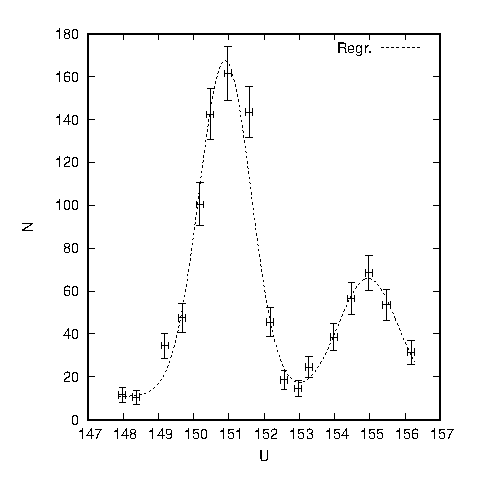
\includegraphics[width=0.7\textwidth]{data/Ba_fein.eps}
  \caption{Aufgezeichnetes Emissionsspektrum von Barium in Feinmessung}
  \label{fig:ba_fein}
\end{figure}

\begin{figure}[h]
  \centering
  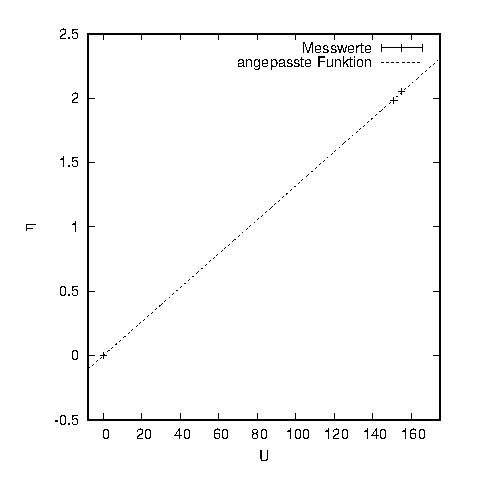
\includegraphics[width=0.7\textwidth]{data/kal.eps}
  \caption{Kalibrationskurve für Zusammenhang von Hallspannung und Elektronenimpuls}
  \label{fig:kal}
\end{figure}

\subsection{Bestimmung des Auflösungsvermögens}
Das Auflösungsvermögen wird für beide Einstellungen (4\% und 1\% Transmission) und beide Emissionlinien von Barium bestimmt. Für die Grobmessung (Daten siehe Tabelle \ref{tab:grob} im Anhang) wird wieder die Funktion aus Gleichung (\ref{eq:gauss}) angepasst. Die Parameter sind
\begin{align*}
  A_0&=5\pm 3\\
  A_1&=175\pm 15\\
  A_2&=79\pm 12\\
  \mu_1&=151,3 \pm 0,1\\
  \mu_2&=155,2 \pm 0,2\\
  \sigma_1&=0,38 \pm 0,06\\
  \sigma_2&=0,6 \pm 0,2.
\end{align*}
Die Funktion ist in Abbildung \ref{fig:ba_grob} zu sehen.\\

Das Auflösungsvermögen ist definiert als
\begin{align*}
  R=\frac{\delta\eta}{\eta}=\frac{\delta U}{U},
\end{align*}
wobei $\delta\eta$ für den Abstand zu $\eta$ steht, bei dem die aufgenommene Zahl der Teilchen sich halbiert. Da Impulse und Spannungen zueinander proportional sind ist keine Umrechnung von Impulsen und Spannungen notwendig. Mit den angepassten Gaußkurven gilt also 
\begin{align*}
  R=\frac{\sqrt{\log(2)} \sigma}{\mu}.
\end{align*}
Die berechneten Auflösungsvermögen sind in Tabelle \ref{tab:aufloesung} zu sehen. Die Auflösung ist besser ($R$ kleiner) bei den Messungen mit größerer Transmissionsrate. Dies entspricht nicht dem erwarteten Verhalten. Bei kleinerer (größerer) Transmission ist die Auflösung der L-Linie (K-Linie) besser.

\begin{table}[h]
    \centering
    \caption{Auflösungsvermögen von Spektrometer}
    \label{tab:aufloesung}
    \begin{tabular}{c | c c}
      \toprule
       $R/ \%$ & 1\% Transmission & 4\% Transmission \\
      \midrule
      K-Linie & $6,43 \pm 0,06$ & $4,17 \pm 0,03$\\
      L-Linie & $5,6 \pm 0,1$ & $5,2 \pm 0,1$\\
      \bottomrule
    \end{tabular}
  \end{table}

\begin{figure}[h]
  \centering
  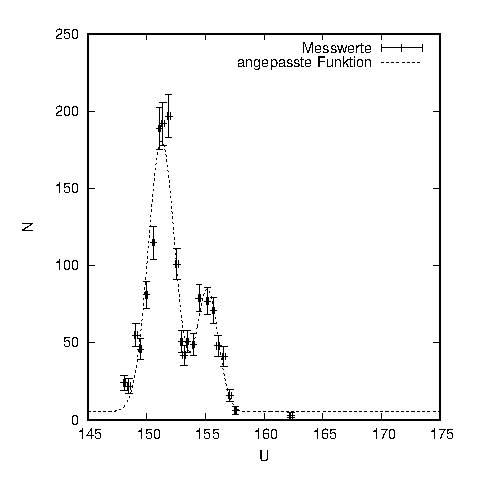
\includegraphics[width=0.7\textwidth]{data/Ba_grob.eps}
  \caption{Aufgezeichnetes Emissionsspektrum von Barium in Grobmessung}
  \label{fig:ba_grob}
\end{figure}
